\documentclass{article}
\usepackage{amsmath,amsthm,amssymb,amsfonts}
\usepackage{setspace,enumitem}
\usepackage{graphicx}
\usepackage{hyperref}
\usepackage{natbib}
\usepackage{afterpage}
\usepackage{xcolor}
\usepackage{etoolbox}
\usepackage{booktabs}
\usepackage{pdfpages}
\usepackage{multicol}
\usepackage{geometry}
\usepackage{accents}
\usepackage{bbm}
\usepackage{placeins}
\hypersetup{
	colorlinks,
	linkcolor={blue!90!black},
	citecolor={red!90!black},
	urlcolor={blue!90!black}
}

\newtheorem{theorem}{Theorem}
\newtheorem{assumption}{Assumption}
\newtheorem{definition}{Definition}
\newtheorem{lemma}{Lemma}
\setlength{\parindent}{0cm}
\geometry{margin = 1in}

\newcommand{\R}{\mathbb{R}}
\newcommand{\ubar}[1]{\underaccent{\bar}{#1}}
\newcommand{\Int}{\text{Int}}
\newcommand{\xbf}{\mathbf{x}}
\newcommand{\Abf}{\mathbf{A}}
\newcommand{\Bbf}{\mathbf{B}}
\newcommand{\Gbf}{\mathbf{G}}
\newcommand{\bbf}{\mathbf{b}}
\newcommand{\one}{\mathbbm{1}}

\newtoggle{extended}
\settoggle{extended}{false}

\title{ECON 810: Homework 4}
\author{Alex von Hafften }

\begin{document}

\maketitle

\section{Data}

In this data assignment you will plot moments from the earnings distribution over the life-cycle similar to Huggett, Ventura, and Yaron [2011]. Using your PSID data from 1978 to 1997 create the following graphs using the approach of Huggett, Ventura, and Yaron [2011] to recover the age effects on the following statistics:

\begin{enumerate}

\item The standard deviation of log earnings as a function of age.

\item The skewness of log earnings as a function of age.

\item The kurtosis of log earnings as a function of age.

\end{enumerate}

I use the time-effects approach.  The chart is below:

\begin{center}
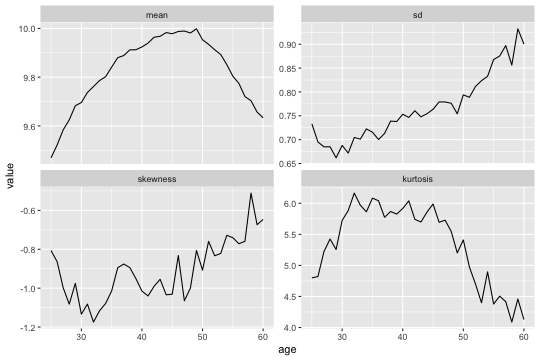
\includegraphics[scale = 0.75]{part_1}
\end{center}

\pagebreak

\section{Model}

\begin{enumerate}

\item  Plot the average path of earnings in the model as well as the standard deviation, skewness and kurtosis of earnings by age. How do these graphs compare data estimates you created in Part (1) and those presented in Huggett, Ventura, and Yaron [2011].

\begin{center}
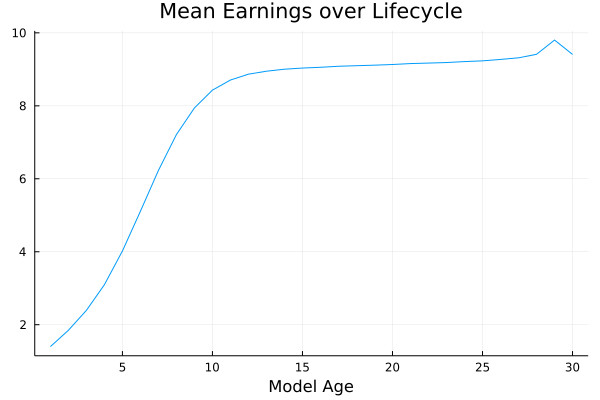
\includegraphics[scale = 0.5]{figure_1_mean}
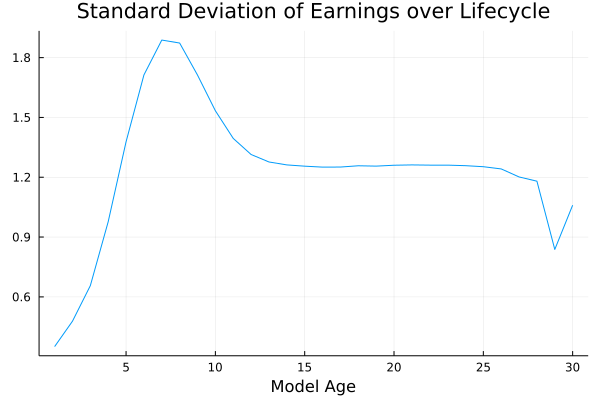
\includegraphics[scale = 0.5]{figure_1_sd}
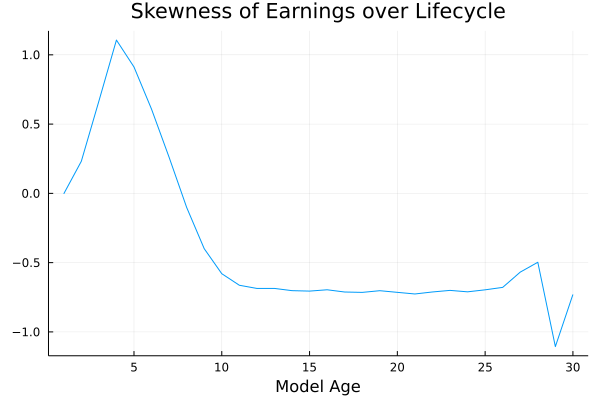
\includegraphics[scale = 0.5]{figure_1_skewness}
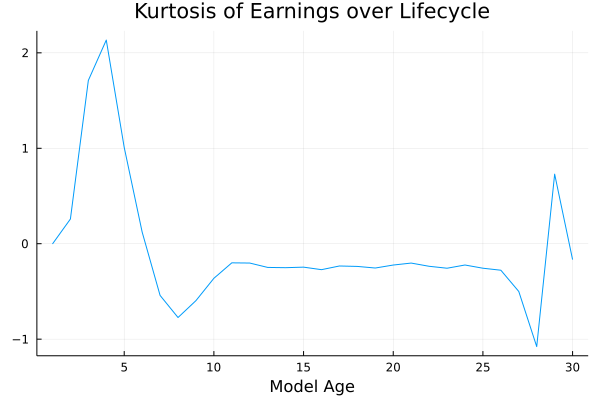
\includegraphics[scale = 0.5]{figure_1_kurtosis}
\end{center}

These graphs look pretty different from both my data estimates in part 1 and HVY.  The hump shape in mean earnings is not really present.  In part 1 and HVY, the standard deviation was steadily increasing with age.  Here, it starts low and peak around model age of 7 and then declines to a steady level for the rest of the lifecycle.  The skewness and kurtosis more-or-less match the standard deviation, but in the data the skewness was steadily increasing and the kurtosis was hump shaped.

\pagebreak

\item Plot the policy function for investing in human capital as a function a function of (1) assets and (2) human capital for workers of different ages.

Here, I plot the policy function for low, medium, and high capital across human capital as well as low, medium, and high human capital across capital for $t=10$ and $t=20$.

\begin{center}
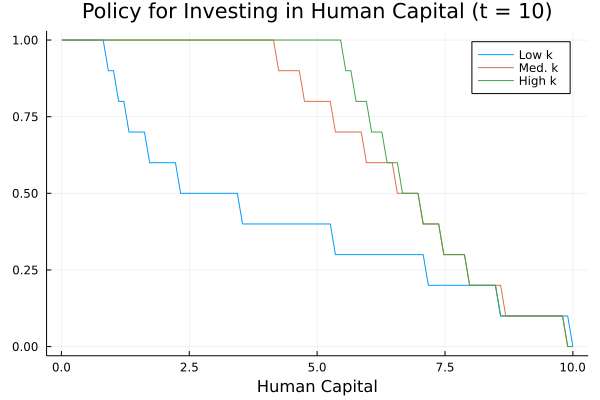
\includegraphics[scale = 0.5]{figure_2_10_pf_h}
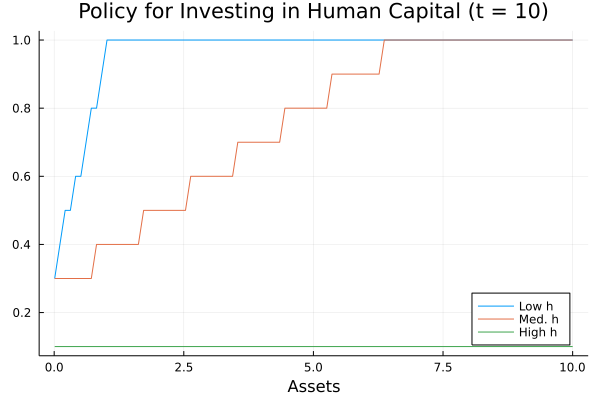
\includegraphics[scale = 0.5]{figure_2_10_pf_k}
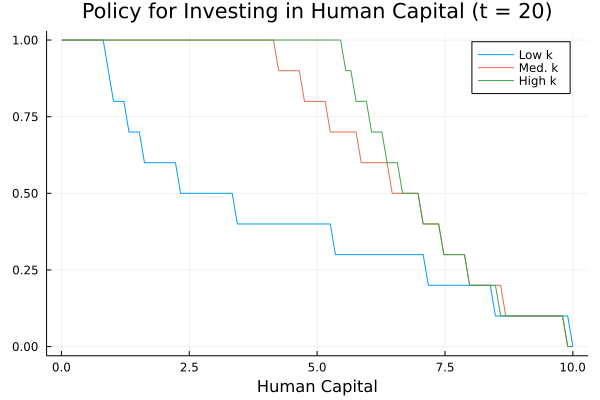
\includegraphics[scale = 0.5]{figure_2_20_pf_h}
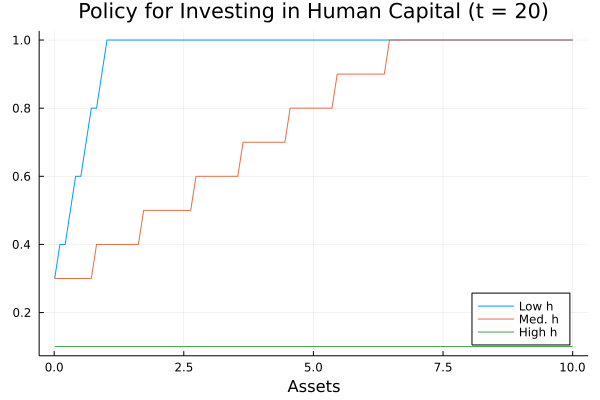
\includegraphics[scale = 0.5]{figure_2_20_pf_k}
\end{center}

\pagebreak

\item How do these policy functions change if you increase the variance of shocks to human capital? Why do you think you see this pattern?

Here, I doubled the variance of the human capital shocks. And create the same plots as problem 2.  Generally, there is lower investment in human capital because it is riskier.

\begin{center}
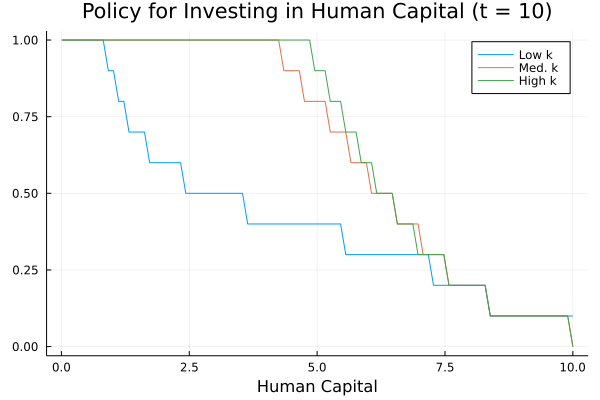
\includegraphics[scale = 0.5]{figure_3_10_pf_h}
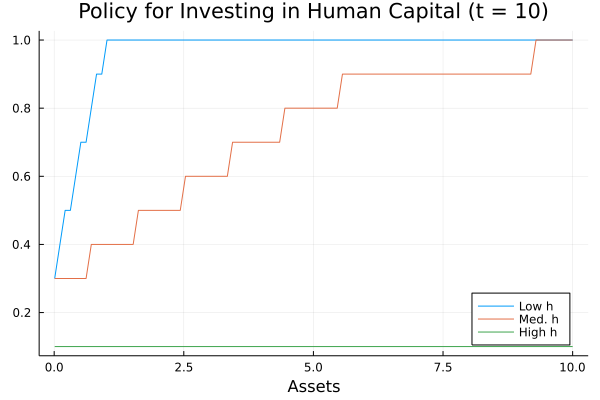
\includegraphics[scale = 0.5]{figure_3_10_pf_k}
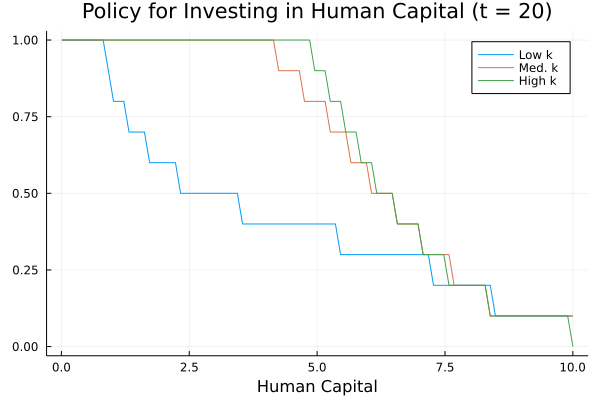
\includegraphics[scale = 0.5]{figure_3_20_pf_h}
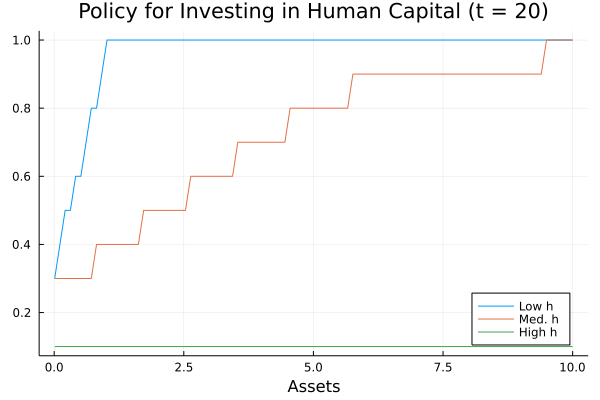
\includegraphics[scale = 0.5]{figure_3_20_pf_k}
\end{center}

\pagebreak

\item Create a measure of lifetime earnings based upon Guvenen et al. [2017]. If you increase the initial dispersion of human capital, how does your measure of lifetime inequality change? How does the path of the standard deviation of earnings by age compare to your graph from part (a)?

I look at a simulations average earning across their lifespan. I plot the histogram across simulations.  The baseline is denoted ``low $\sigma$\_0".  I also estimate and simulate the model with the variance of the initial level of human capital doubled (``high $\sigma$\_0"). Unsurprisingly, the distribution of lifetime earnings is wider with a higher variance of the initial human capital level. I also plot the standard deviation of earnings over the lifecycle.  The results are very different at the beginning, but by model age 20, the initial distribution appears to not make a difference.

\begin{center}
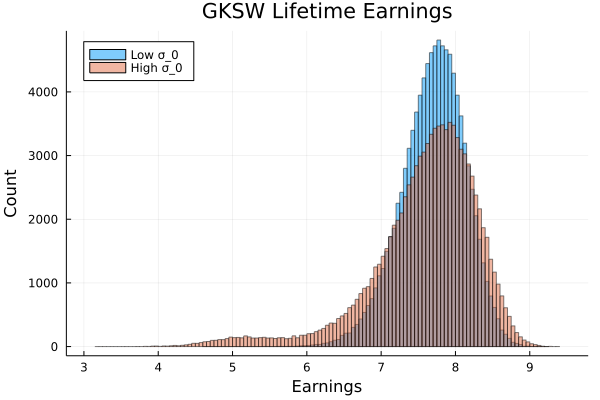
\includegraphics[scale = 0.5]{figure_4_histogram}
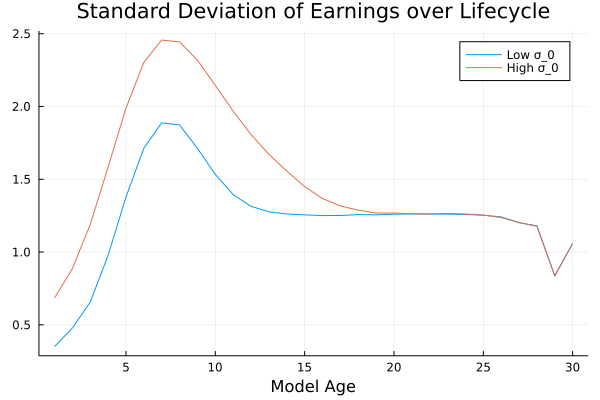
\includegraphics[scale = 0.5]{figure_4_sd}
\end{center}

\end{enumerate}

\end{document}

